\thispagestyle{fancy}
\vspace{\fill}
\subsection{Visão geral dos comandos nas impressoras}
\begin{figure}
    \centering
    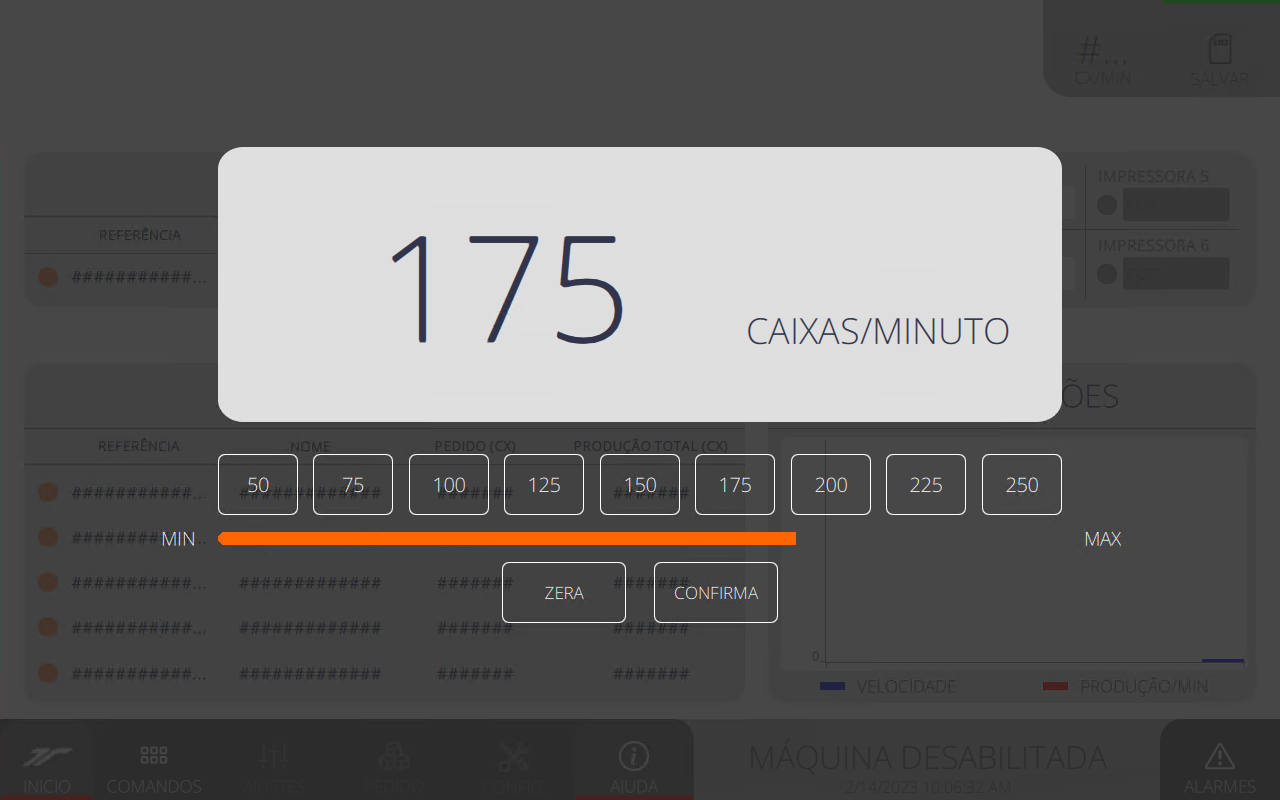
\includegraphics[width=480 px,height=300 px]{src/imagesICV/04-printters/01-printters/commands/1.png}
\end{figure}

\newpage
\thispagestyle{fancy}
\vspace{\fill}
\subsection{Aproximação do anilox bloqueada}
\begin{figure}
    \centering
    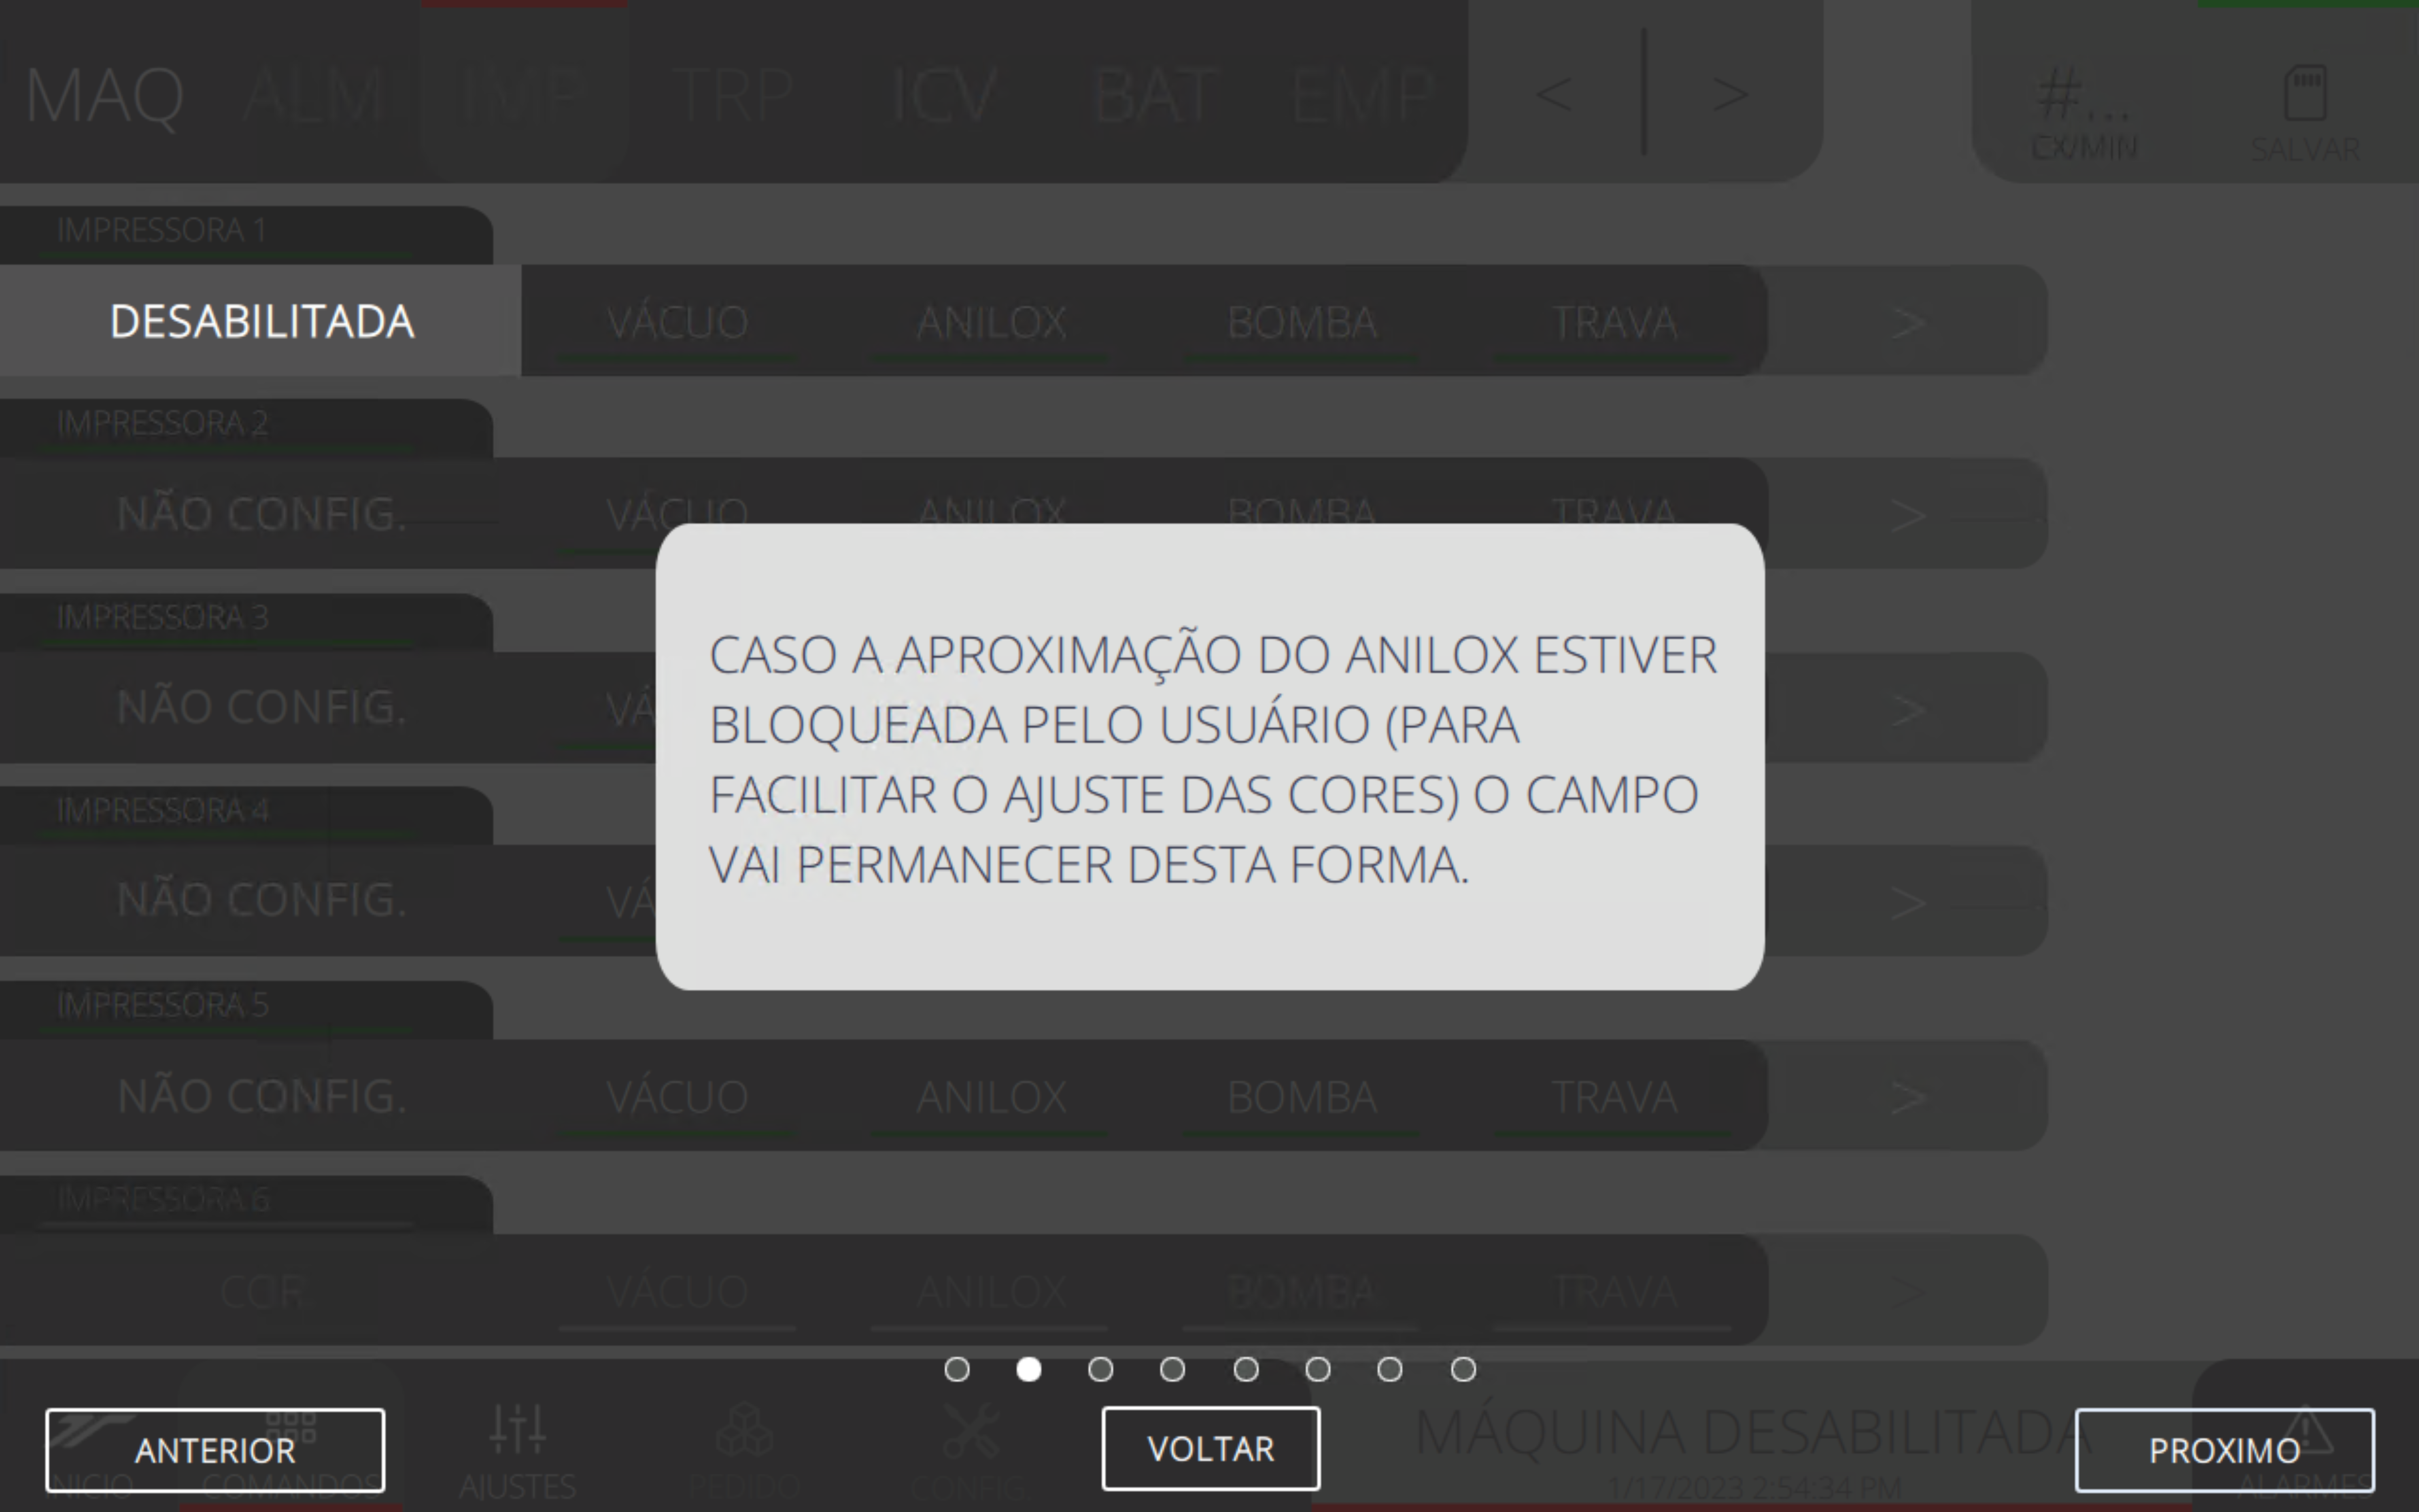
\includegraphics[width=576 px,height=360 px]{src/imagesICV/04-printters/01-printters/commands/2.png}
\end{figure}

\newpage
\thispagestyle{fancy}
\vspace{\fill}
\subsection{Ventilador de vácuo habilitado}
\begin{figure}
    \centering
    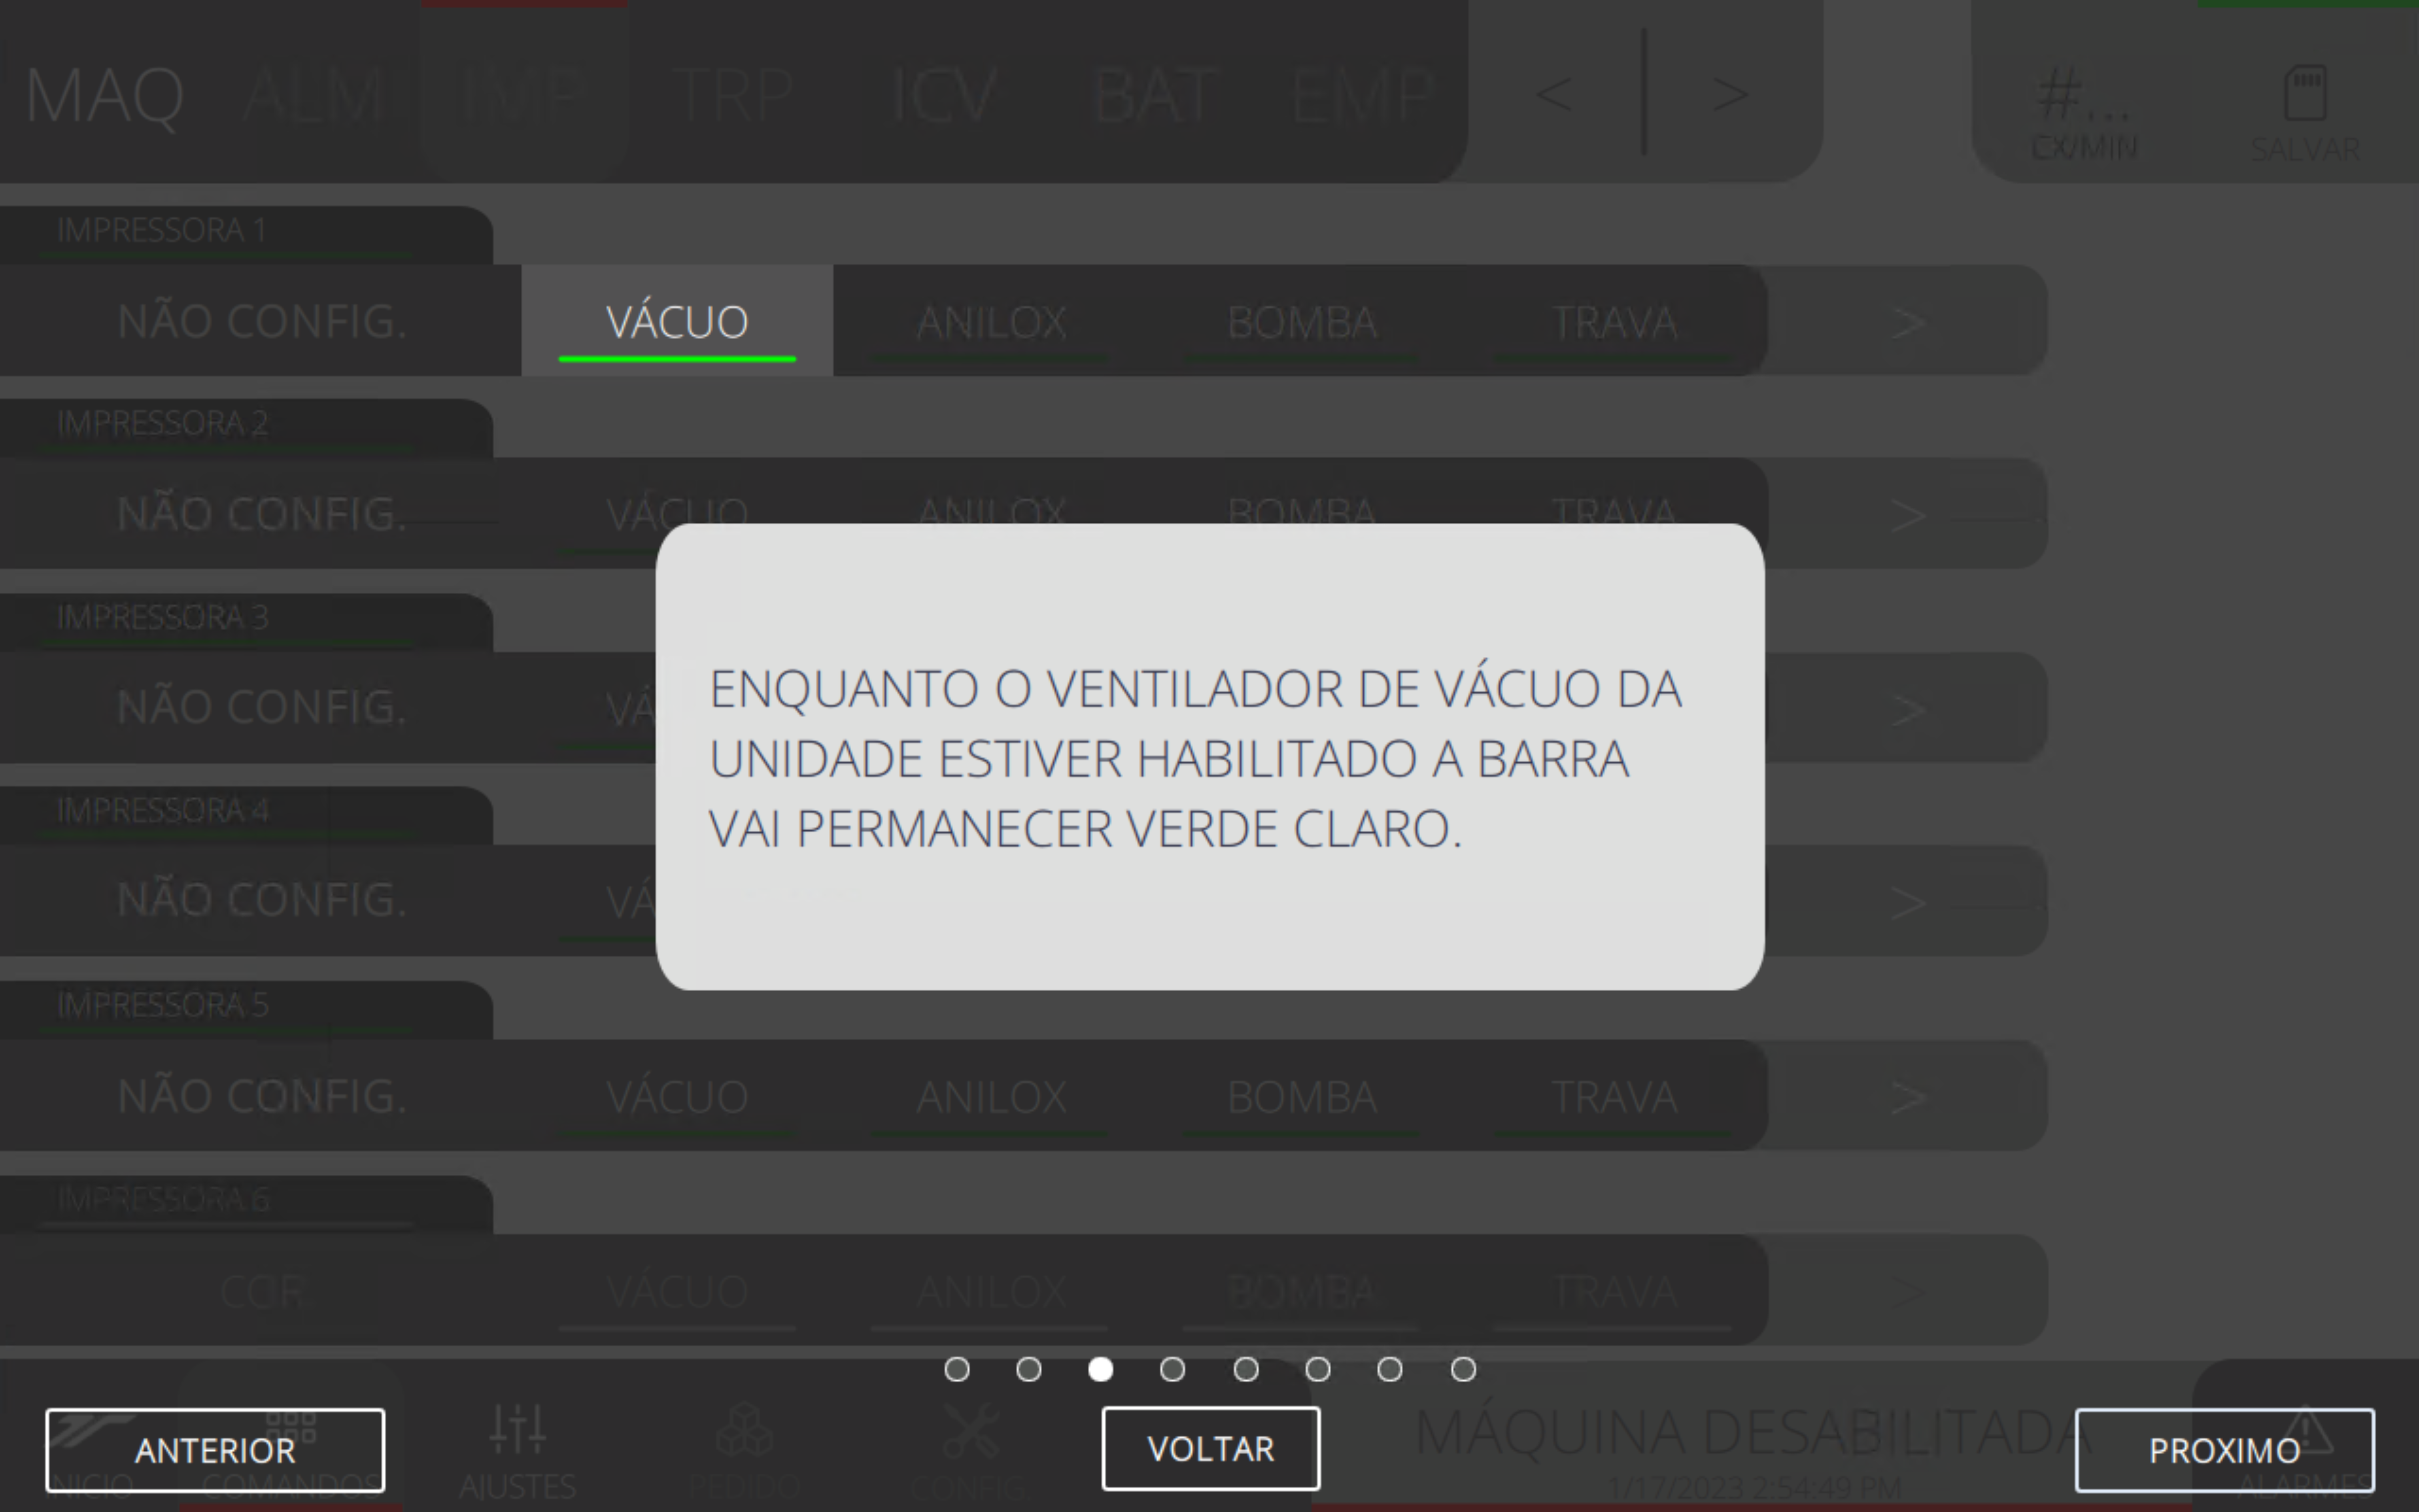
\includegraphics[width=576 px,height=360 px]{src/imagesICV/04-printters/01-printters/commands/3.png}
\end{figure}

\newpage
\thispagestyle{fancy}
\vspace{\fill}
\subsection{Rolo anilox habilitado}
\begin{figure}
    \centering
    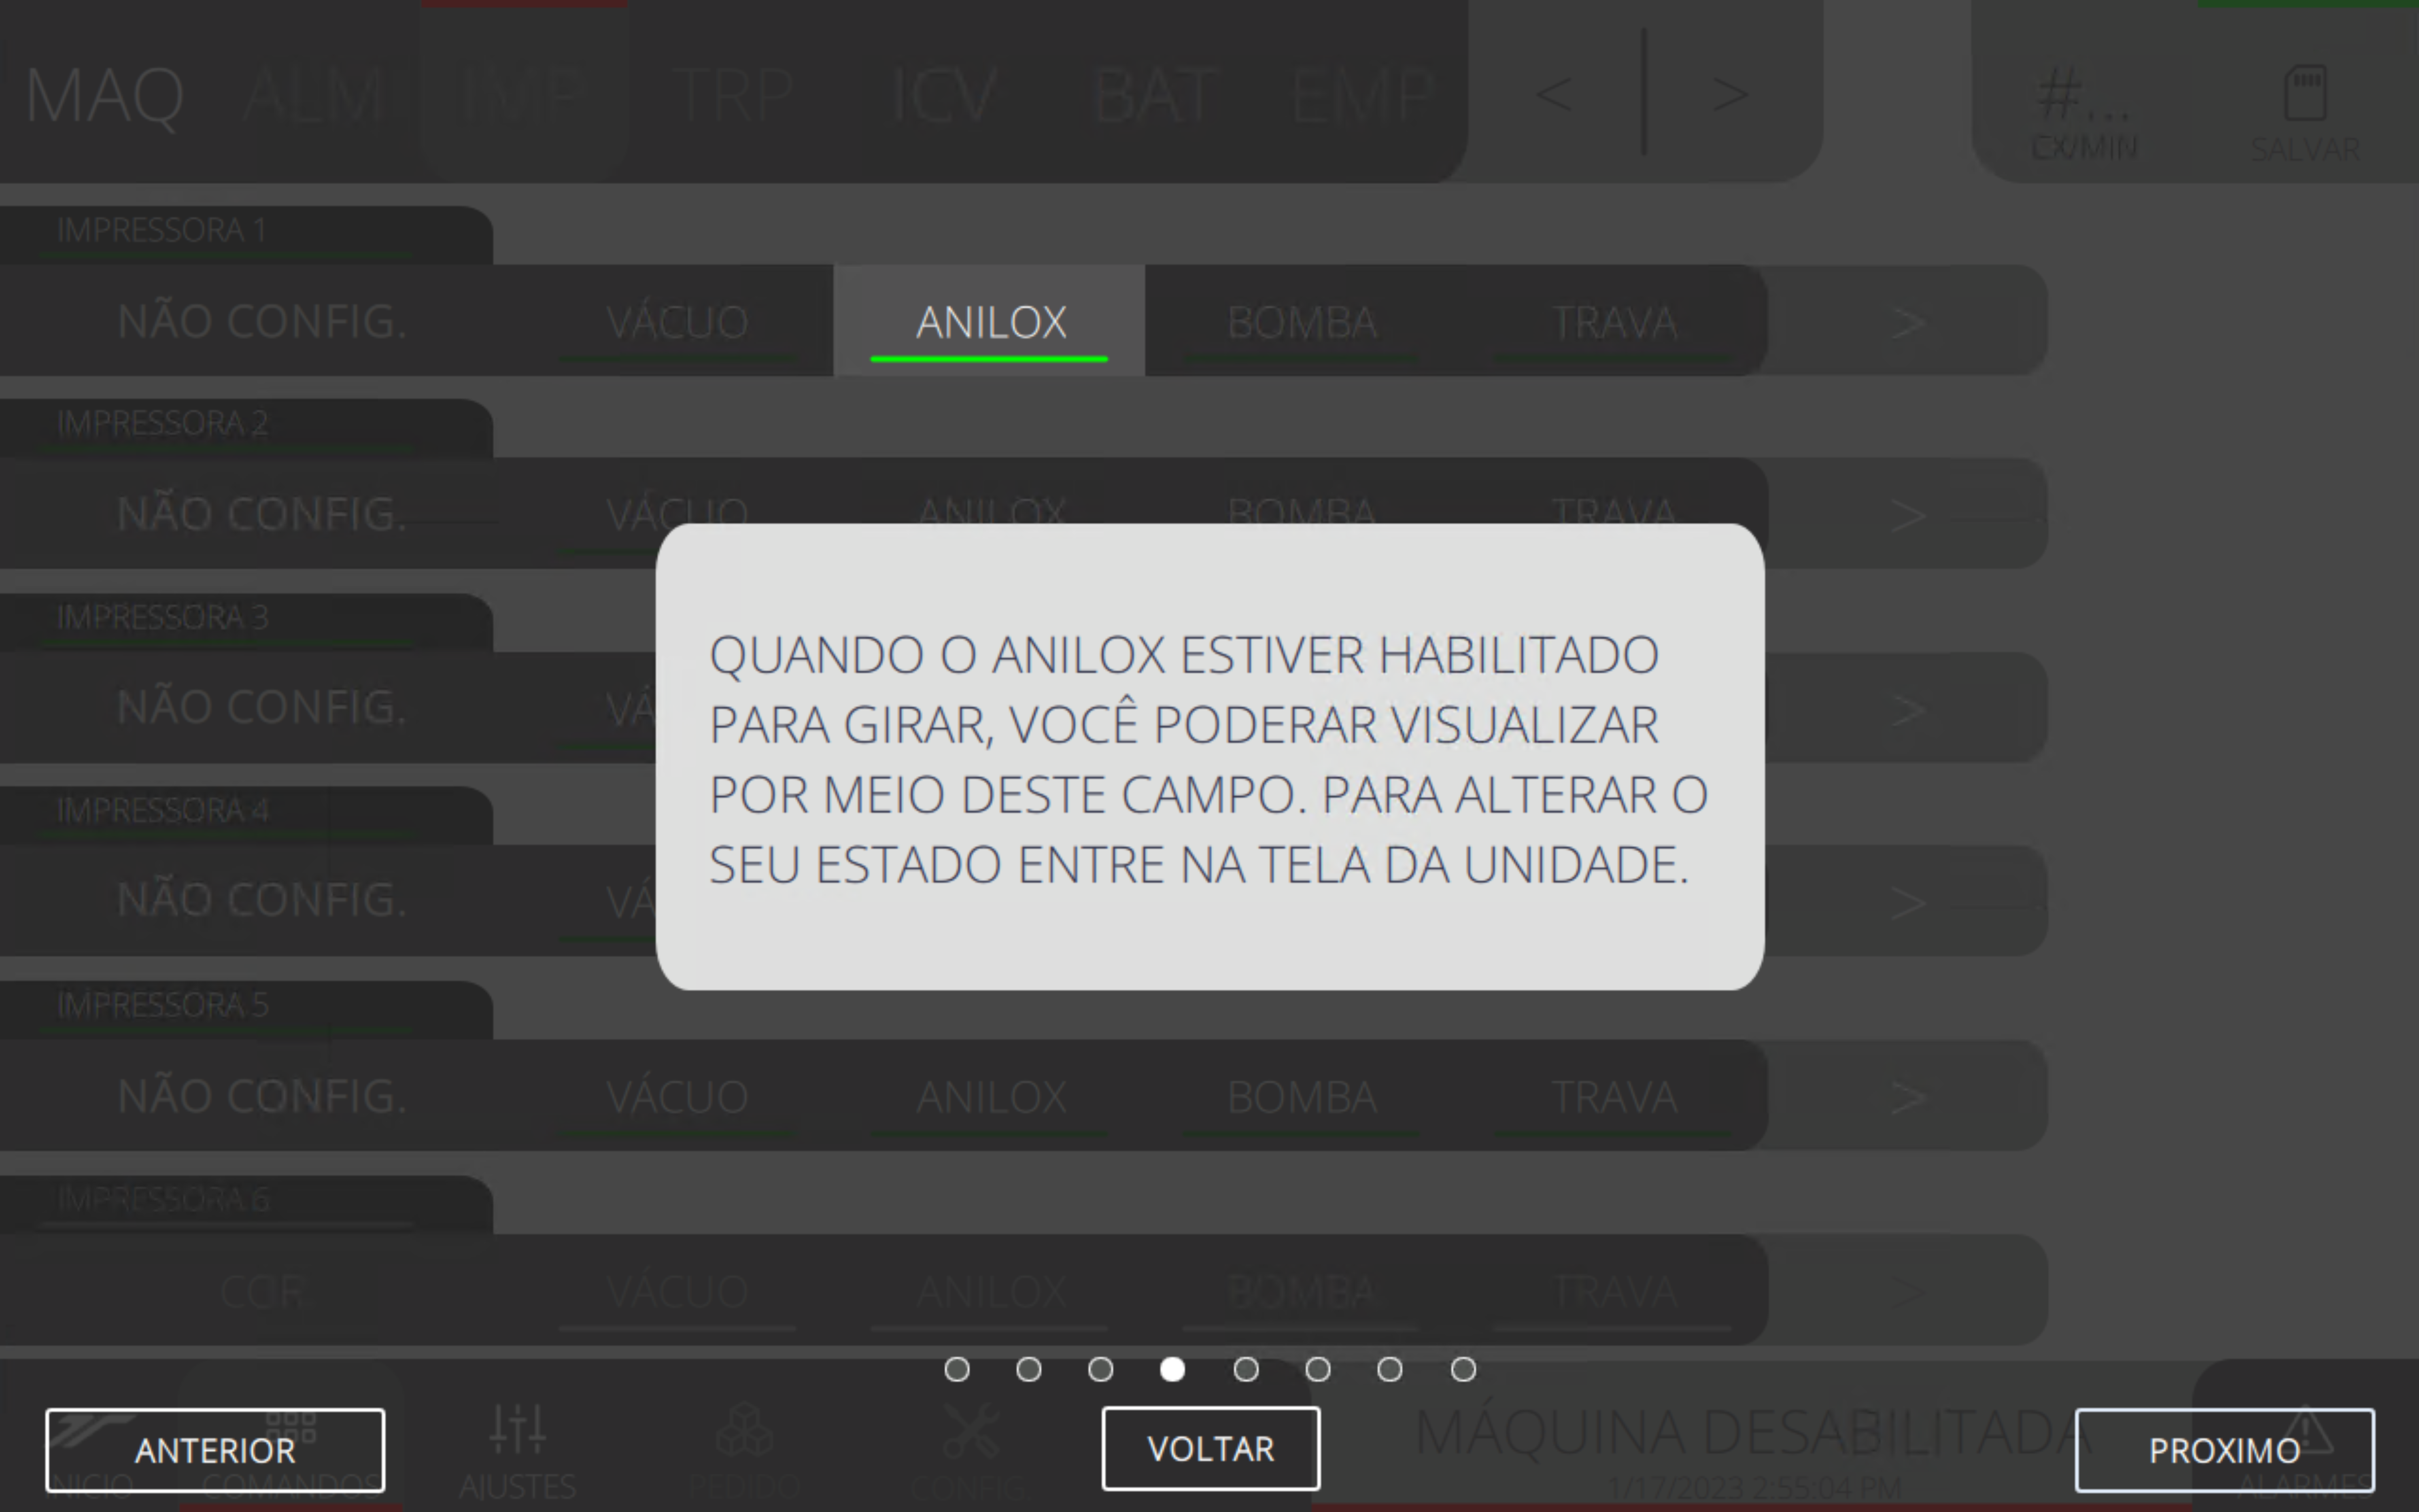
\includegraphics[width=576 px,height=360 px]{src/imagesICV/04-printters/01-printters/commands/4.png}
\end{figure}

\newpage
\thispagestyle{fancy}
\vspace{\fill}
\subsection{Lavagem de tinta habilitada}
\begin{figure}
    \centering
    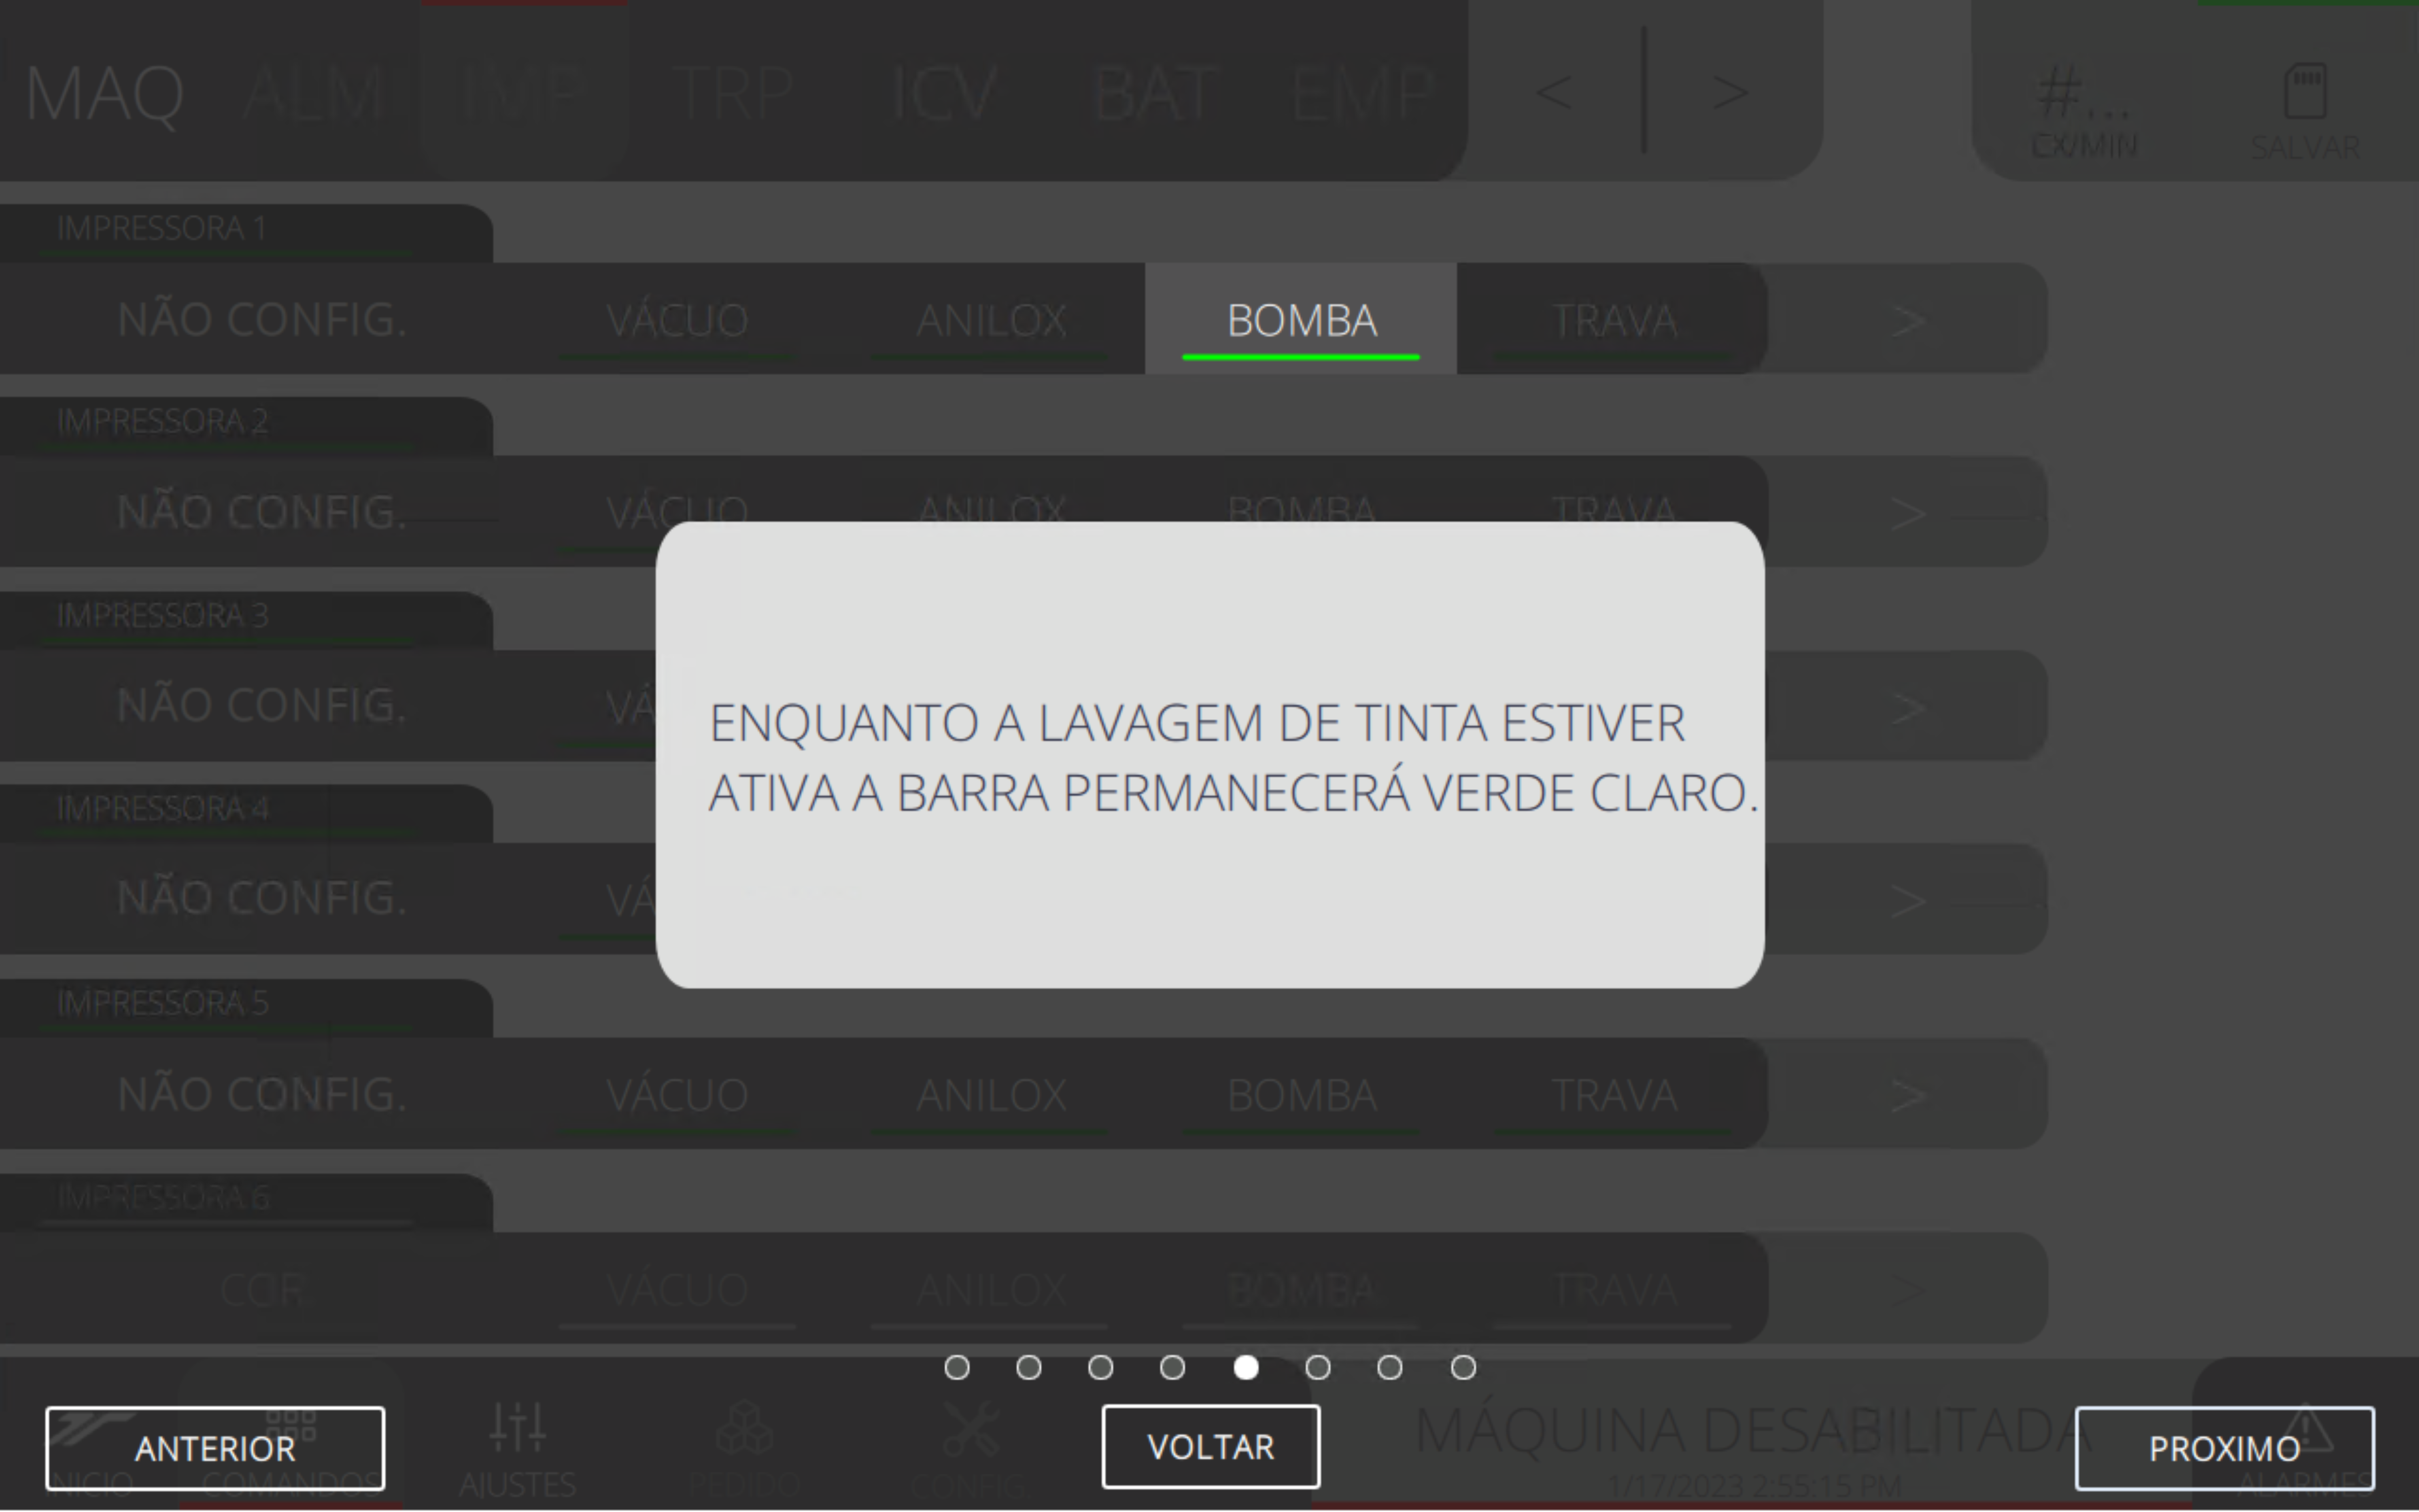
\includegraphics[width=576 px,height=360 px]{src/imagesICV/04-printters/01-printters/commands/5.png}
\end{figure}

\newpage
\thispagestyle{fancy}
\vspace{\fill}
\subsection{Unidade travada}
\begin{figure}
    \centering
    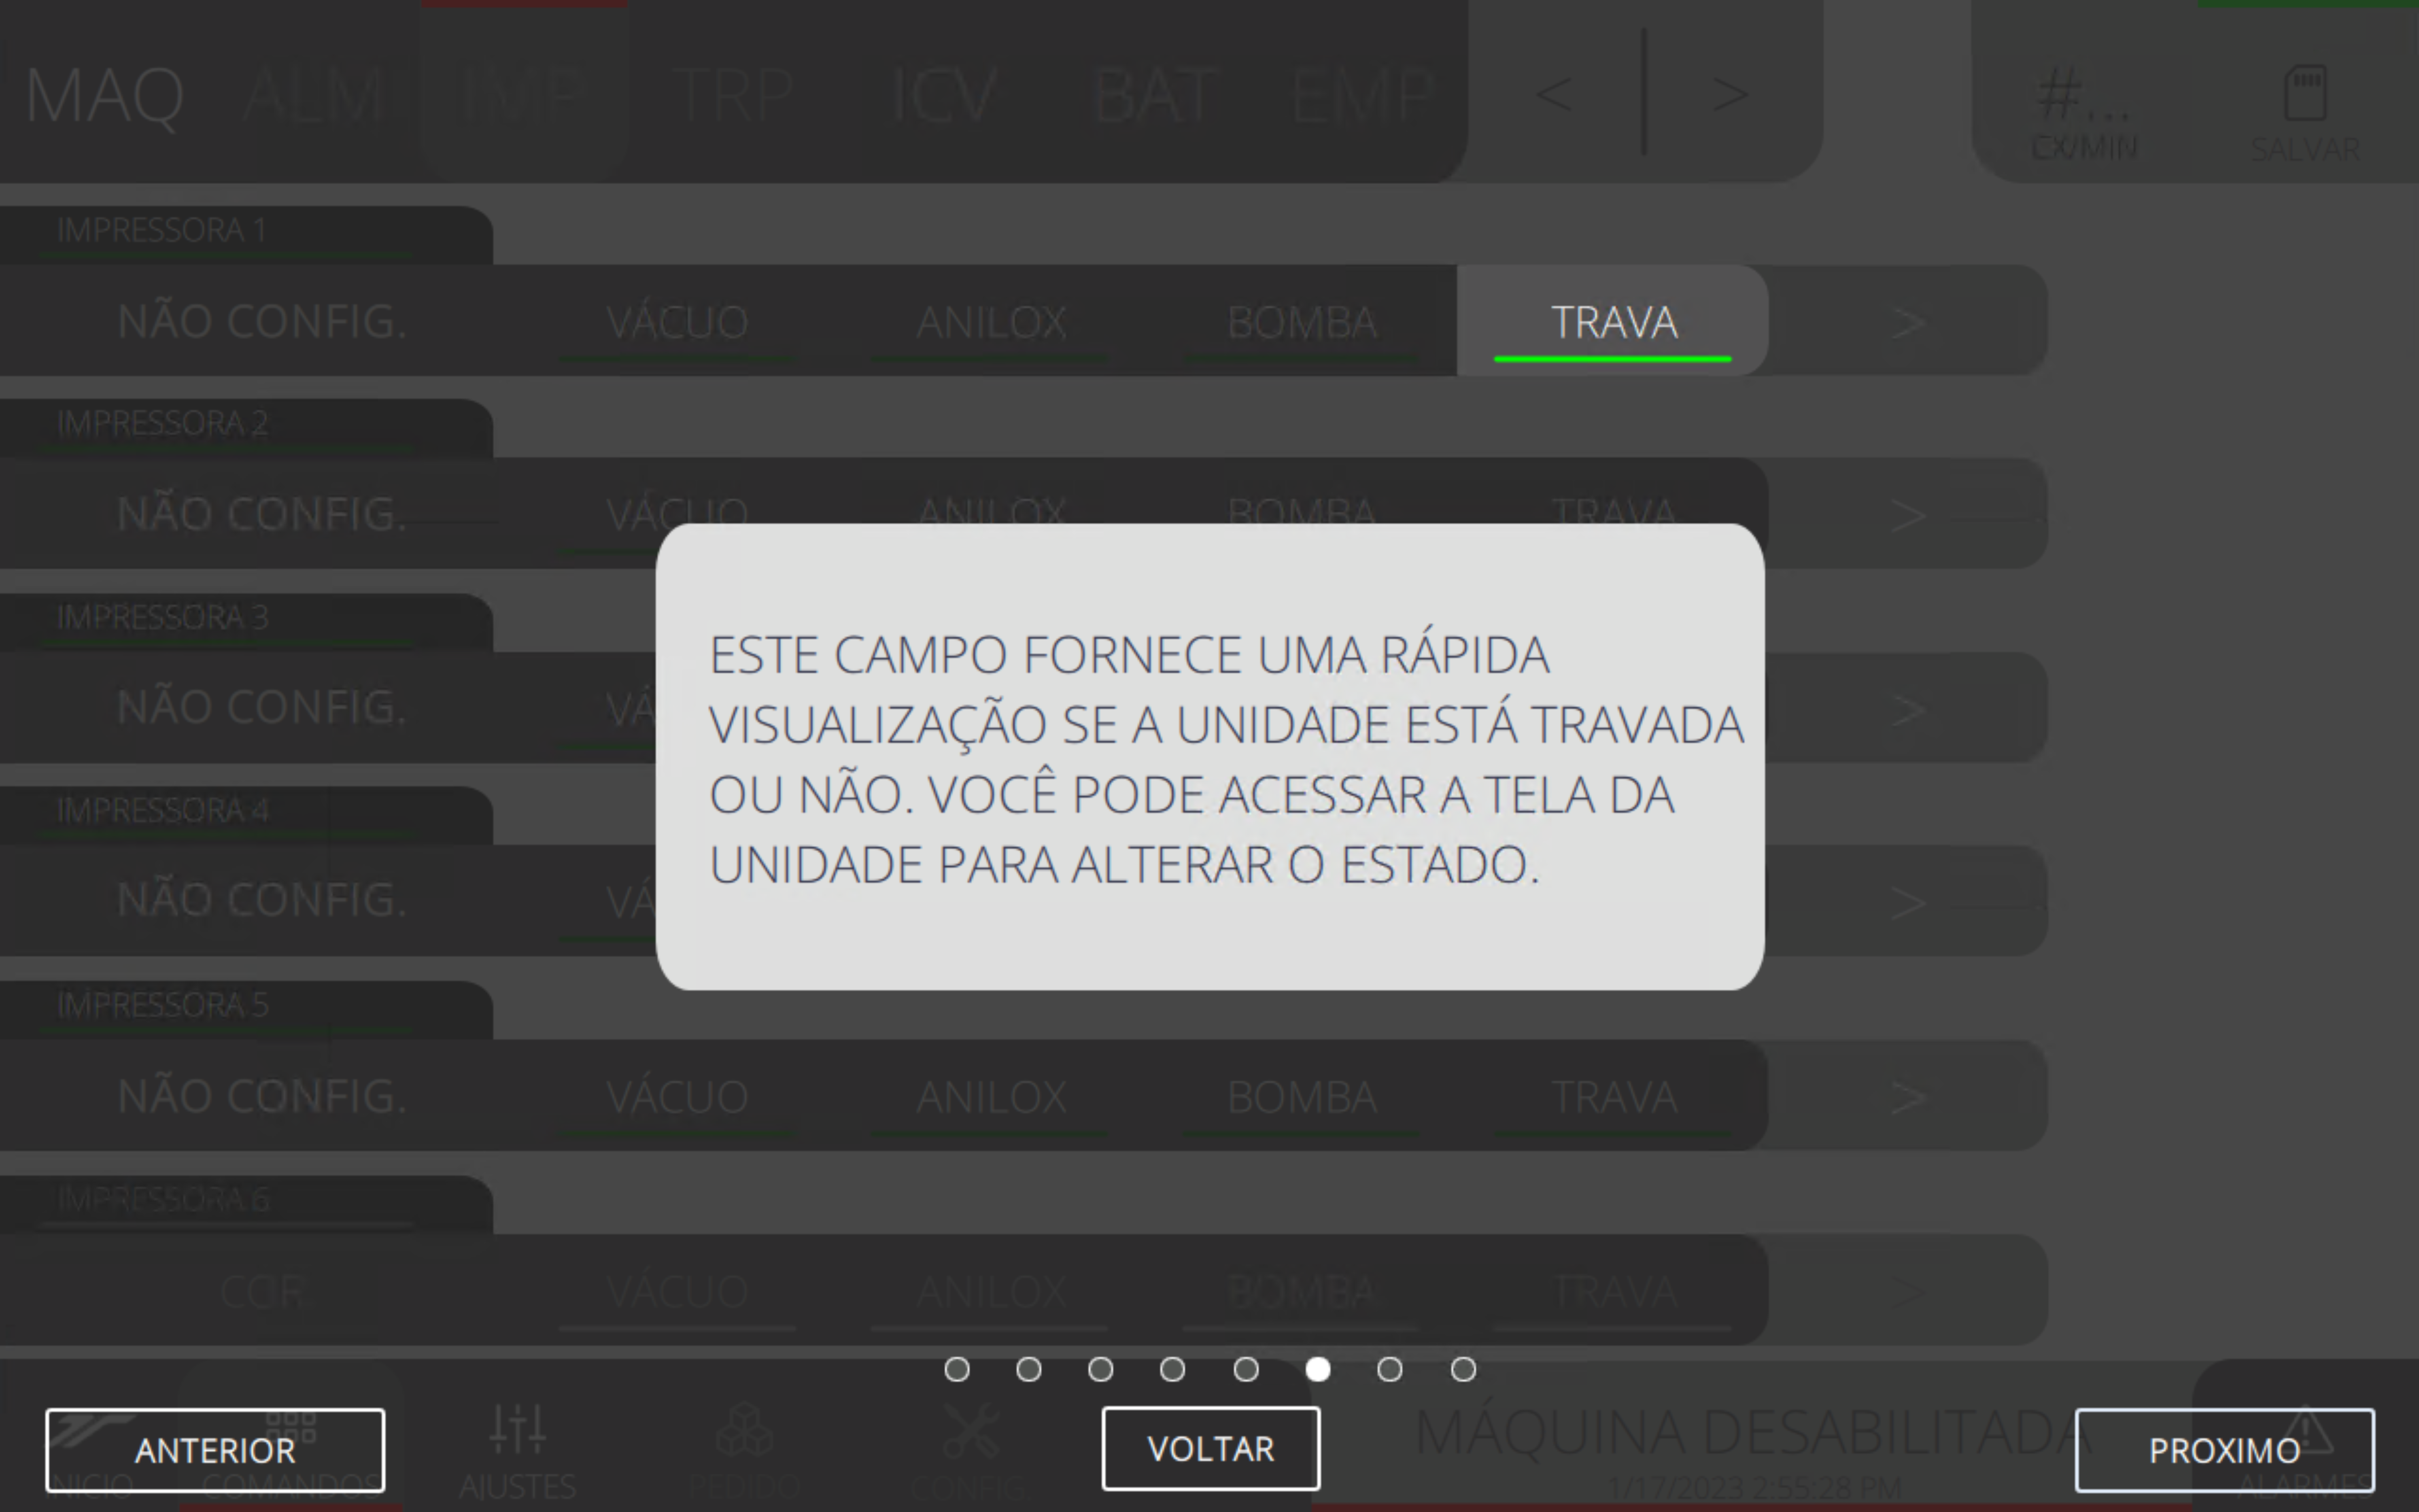
\includegraphics[width=576 px,height=360 px]{src/imagesICV/04-printters/01-printters/commands/6.png}
\end{figure}

\newpage
\thispagestyle{fancy}
\vspace{\fill}
\subsection{Acesso à tela de comamndo da unidade}
\begin{figure}
    \centering
    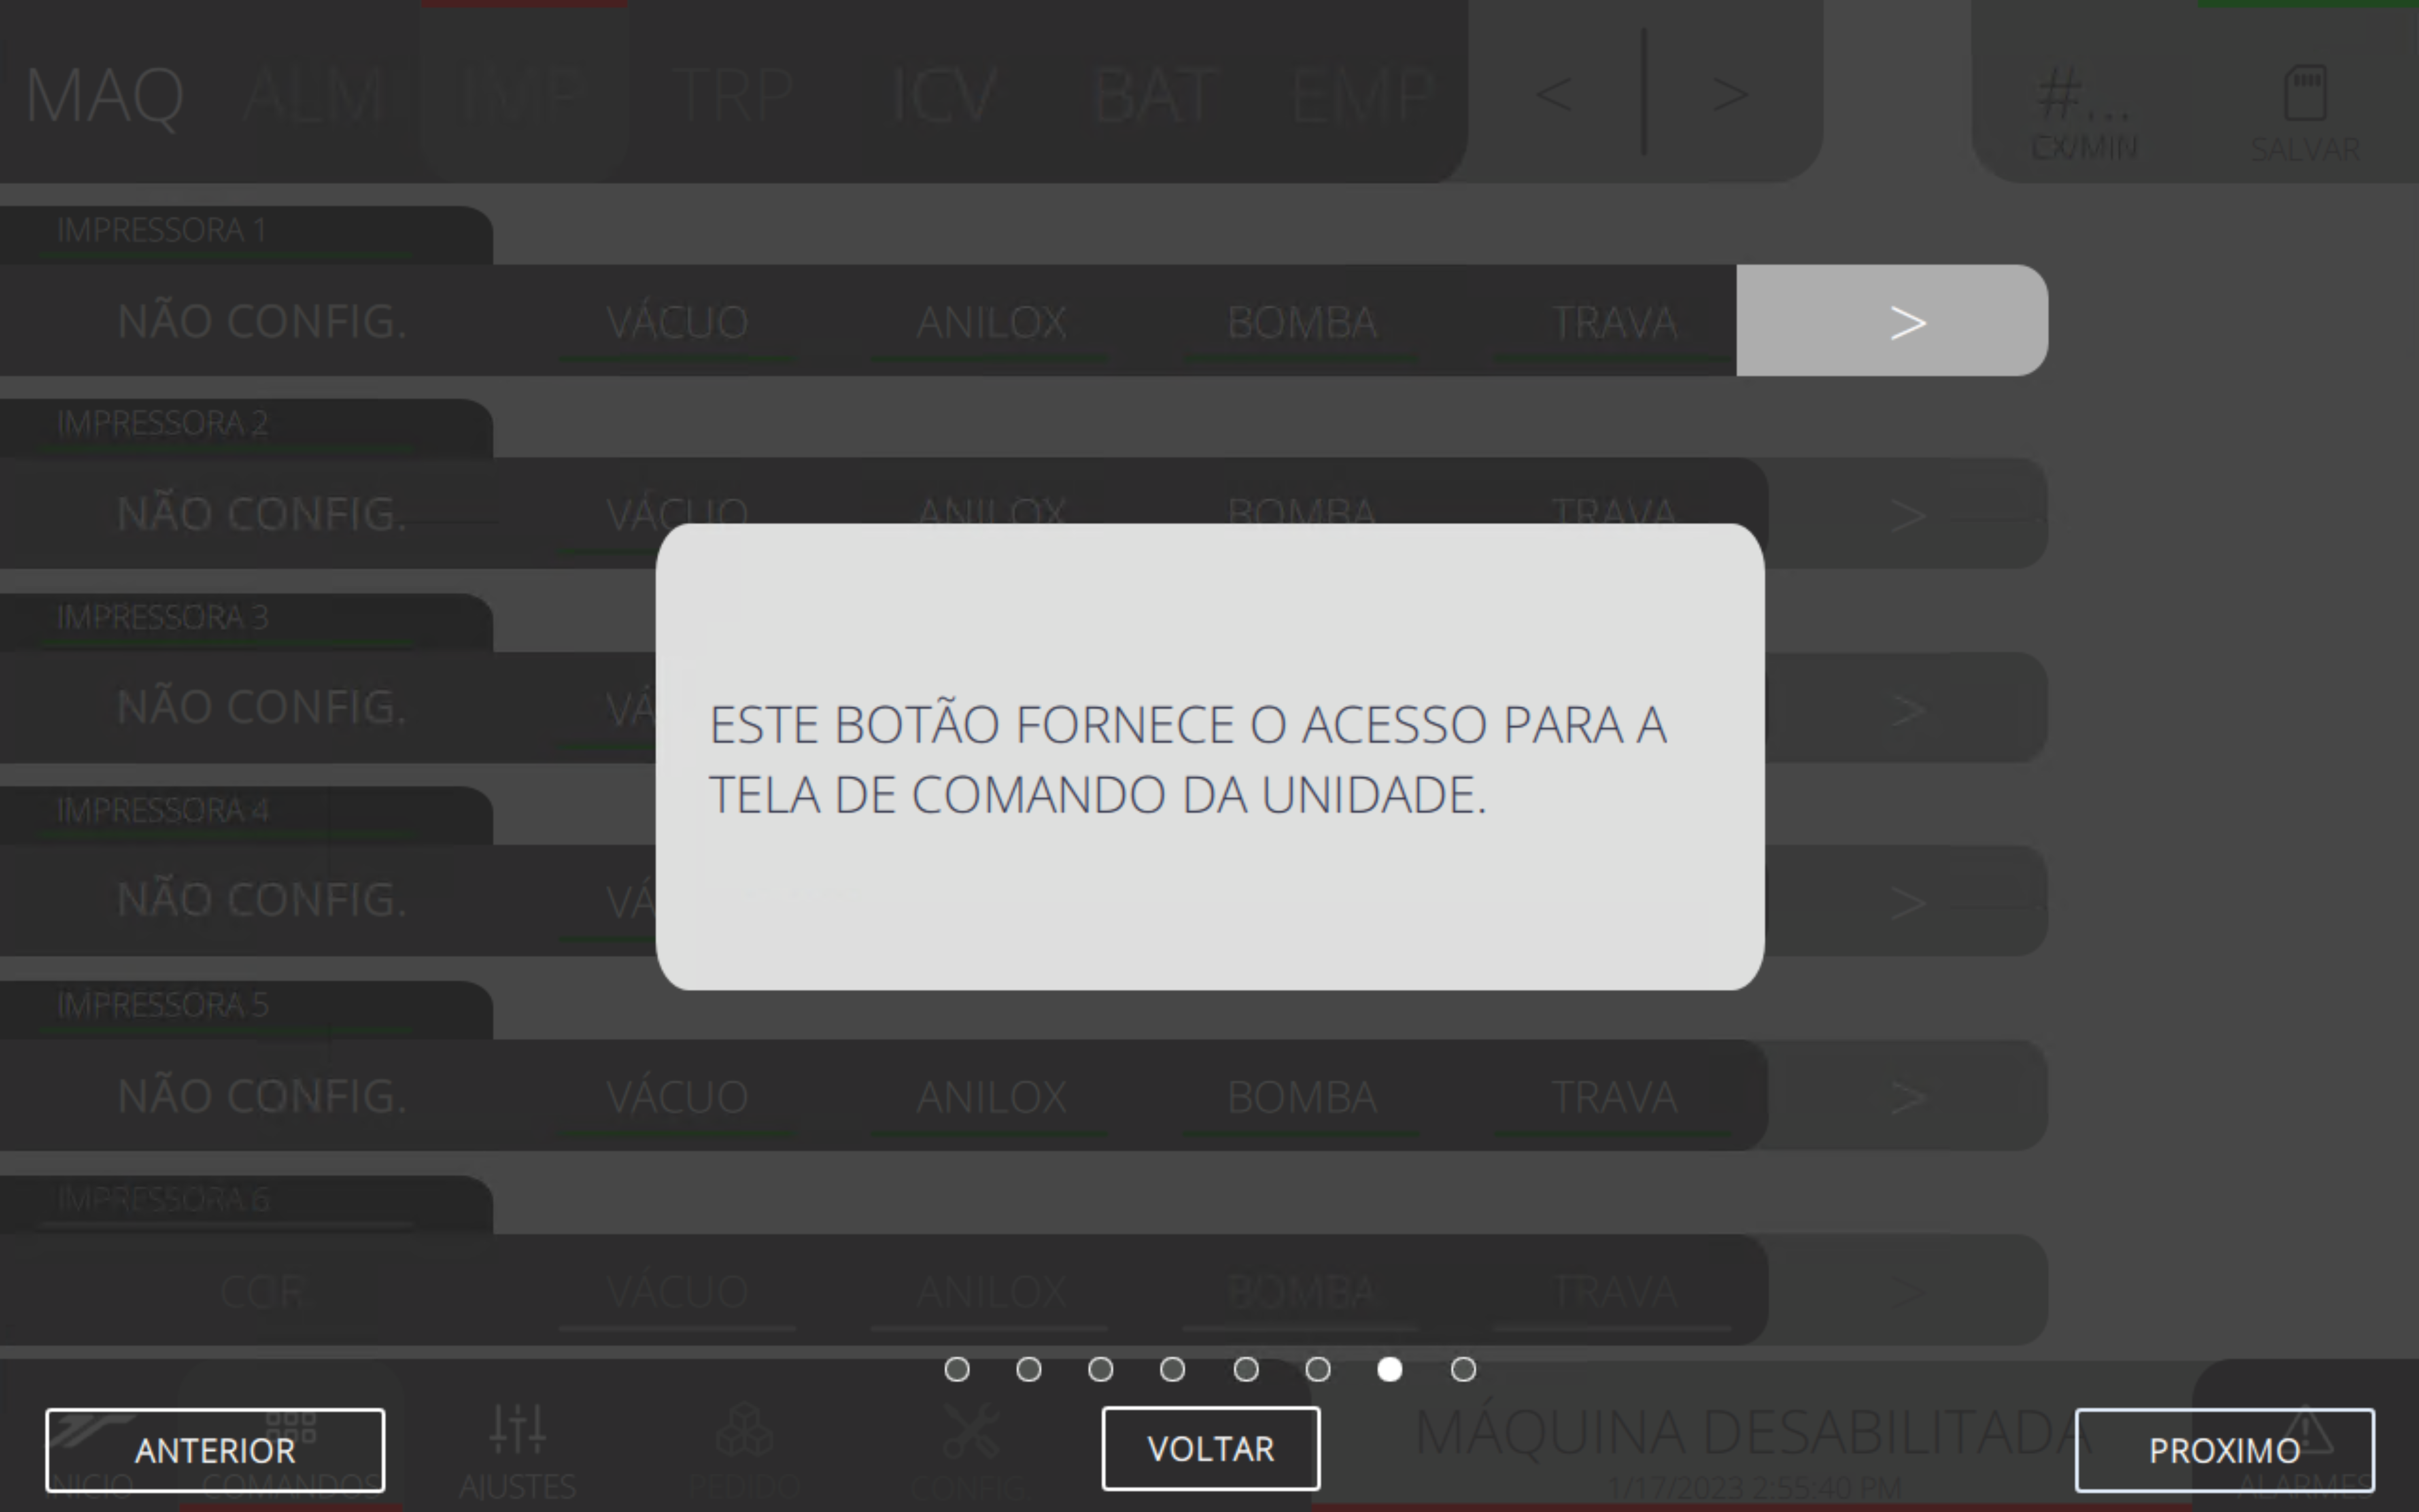
\includegraphics[width=576 px,height=360 px]{src/imagesICV/04-printters/01-printters/commands/7.png}
\end{figure}


